\chapter{Screenshot Proximity System}

In questa sezione illustreremo gli screenshot, sia dell'app che della webapp, delle componenti chiave del nostro prodotto.

\section{App}
\begin{figure}[htpb!]
  \centering
  \subfloat[][\emph{Home page dell'app}.]
  {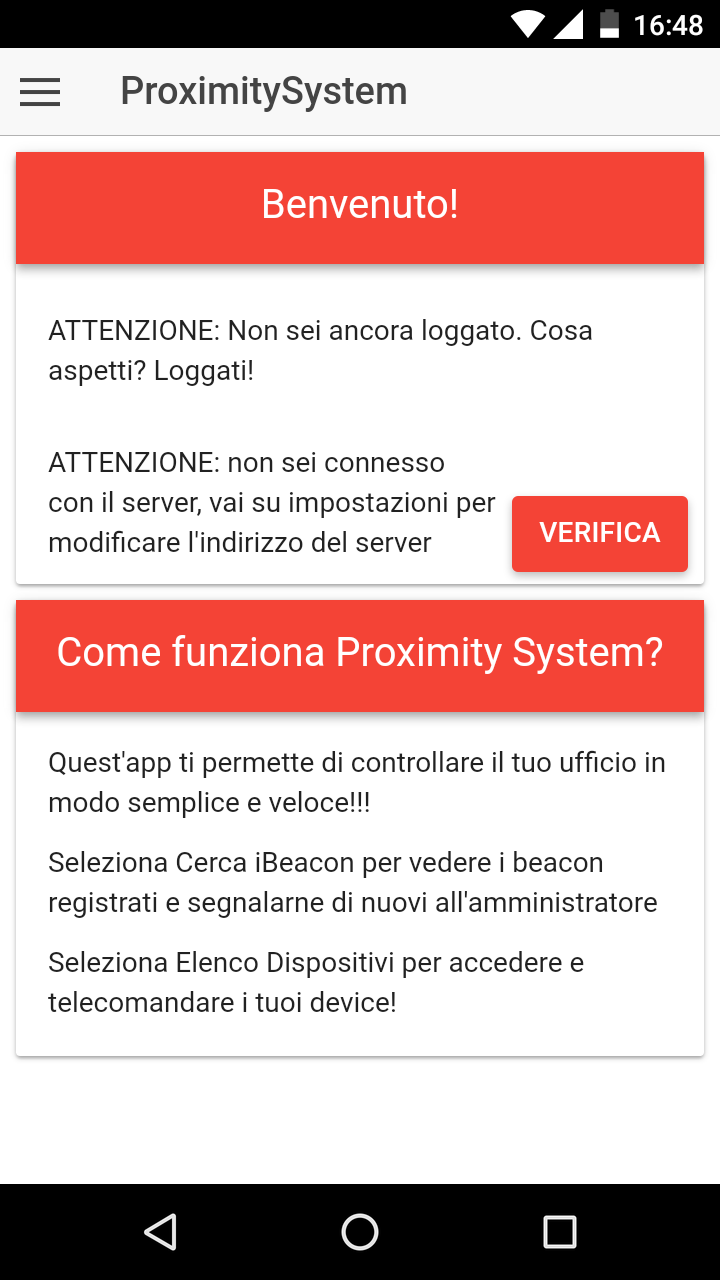
\includegraphics[width=.4\textwidth]{ionic_start}} \quad
  \subfloat[][\emph{Ricerca di server}.]
  {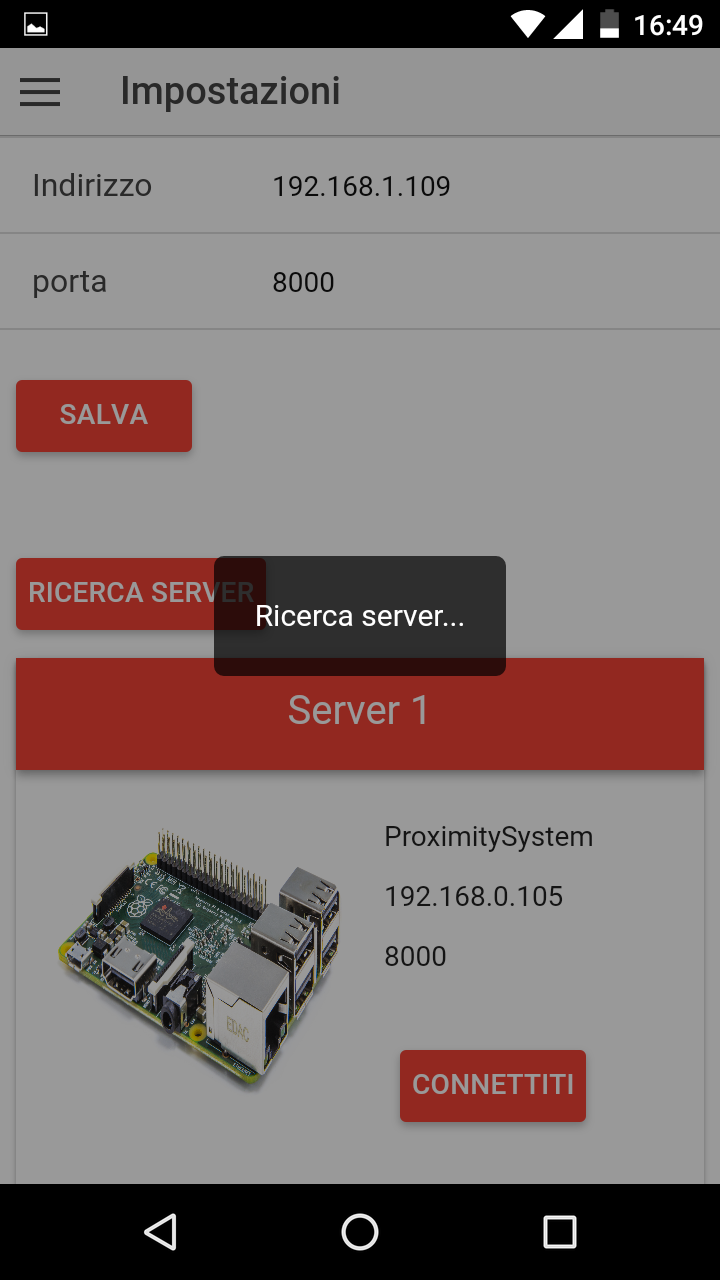
\includegraphics[width=.4\textwidth]{ionic_ricerca}} 
  \caption{Connessione iniziale con il server di Proximity System.}
  \label{fig:subfig}
\end{figure}

\begin{figure}[htpb!]
  \centering
  \subfloat[][\emph{Registrazione nuovo account}.]
  {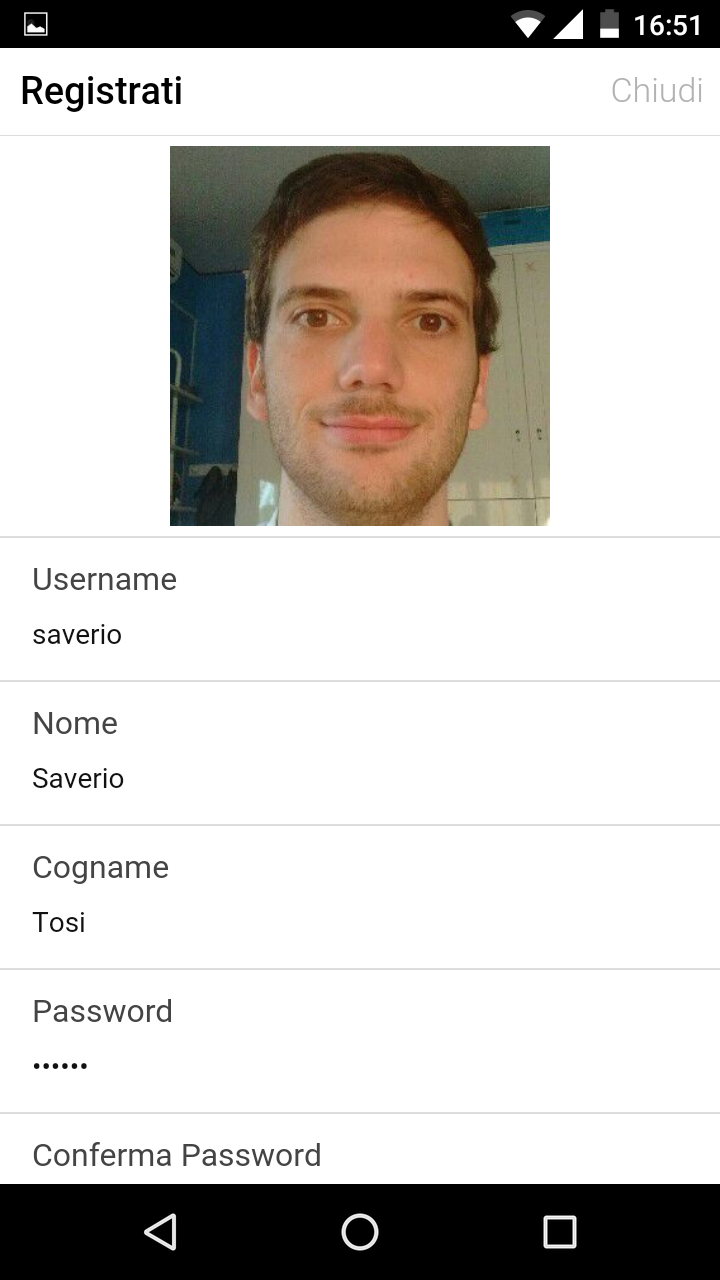
\includegraphics[width=.4\textwidth]{ionic_registrazione}} \quad
  \subfloat[][\emph{Login dall'app}.]
  {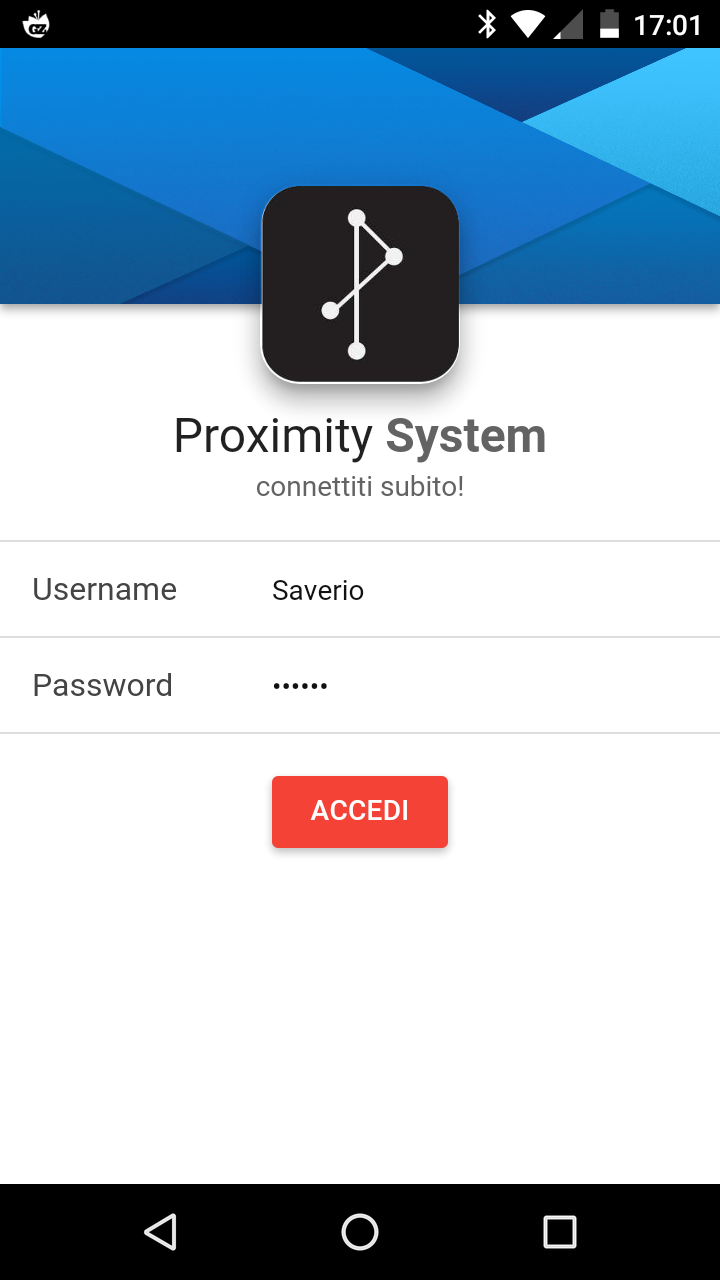
\includegraphics[width=.4\textwidth]{ionic_login}} \\
  \subfloat[][\emph{Ricerca nuovi beacon}.]
  {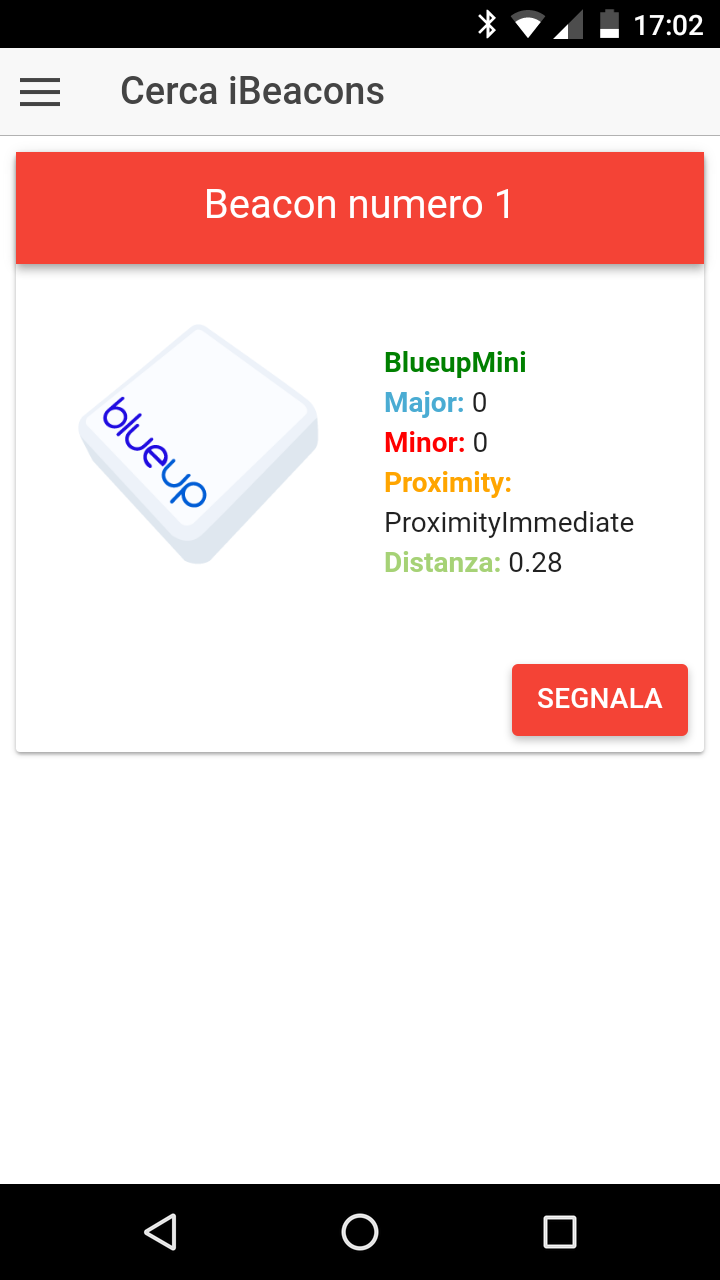
\includegraphics[width=.4\textwidth]{ionic_beacon}} \quad
  \subfloat[][\emph{Elenco dei dispositivi}.]
  {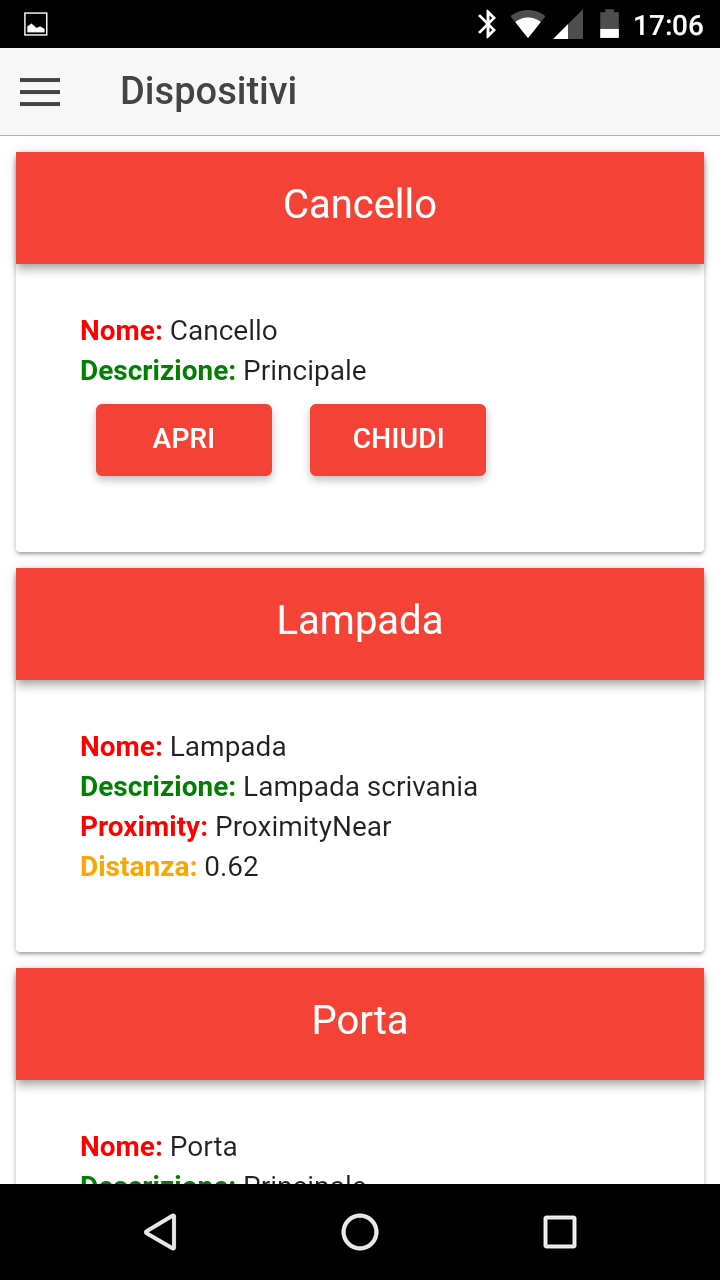
\includegraphics[width=.4\textwidth]{ionic_dispositivi}} 
  \caption{Alcune delle pagine principali dell'app.}
  \label{fig:subfig}
\end{figure}
\newpage
\section{WebApp}

\begin{figure}[htpb!]
  \centering
  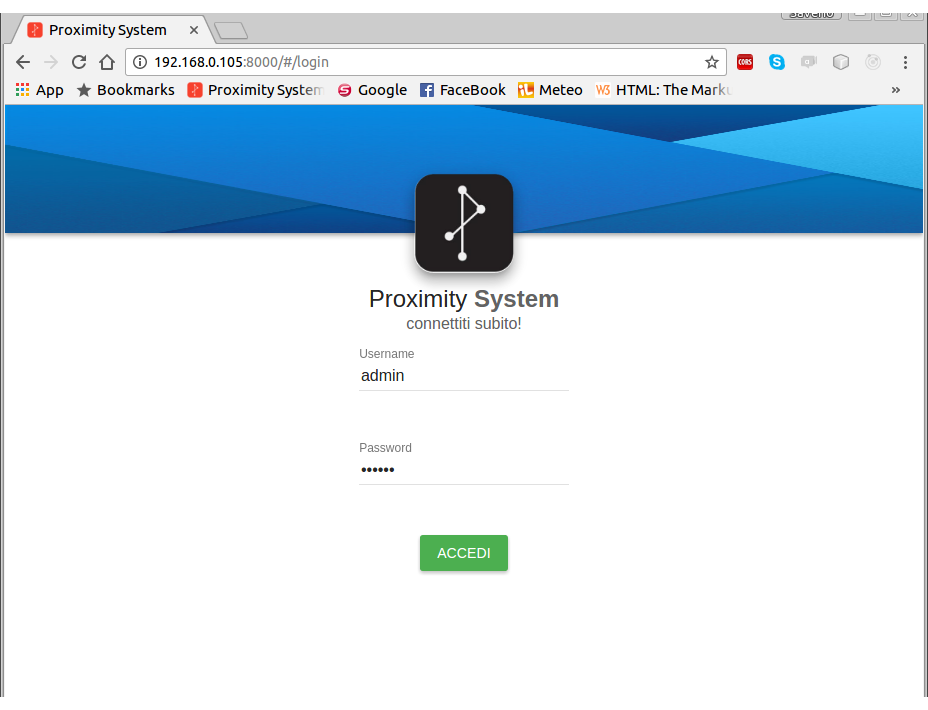
\includegraphics[width=0.8\textwidth]{login}
  \caption{Login da webapp}
  \label{fig:login}
\end{figure}

\begin{figure}[htpb!]
  \centering
  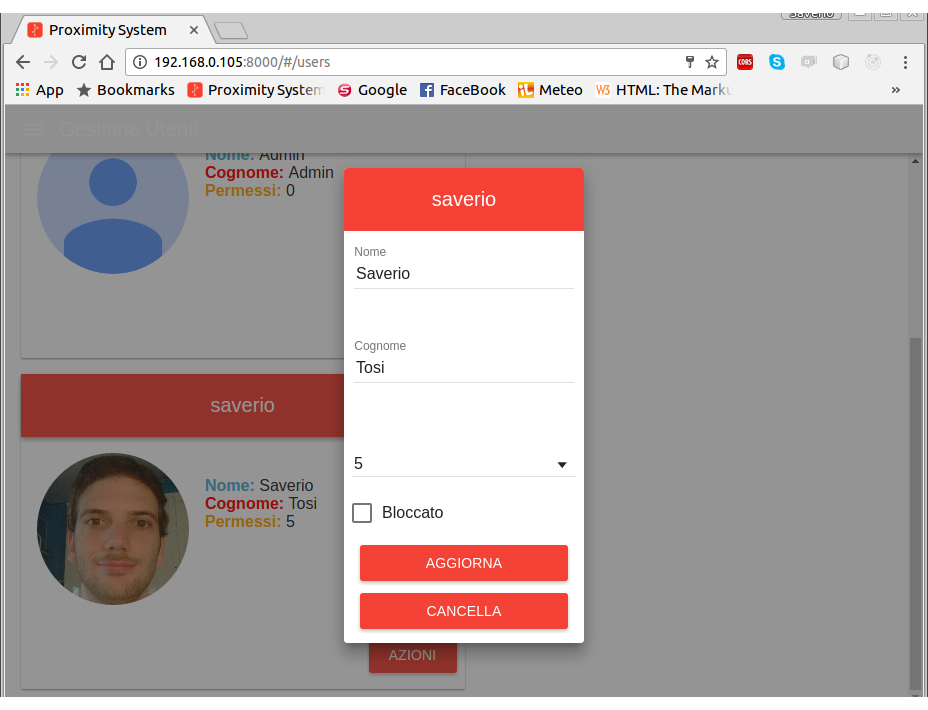
\includegraphics[width=0.8\textwidth]{utenti}
  \caption{Gestione utenti}
  \label{fig:utenti}
\end{figure}

\begin{figure}[htpb!]
  \centering
  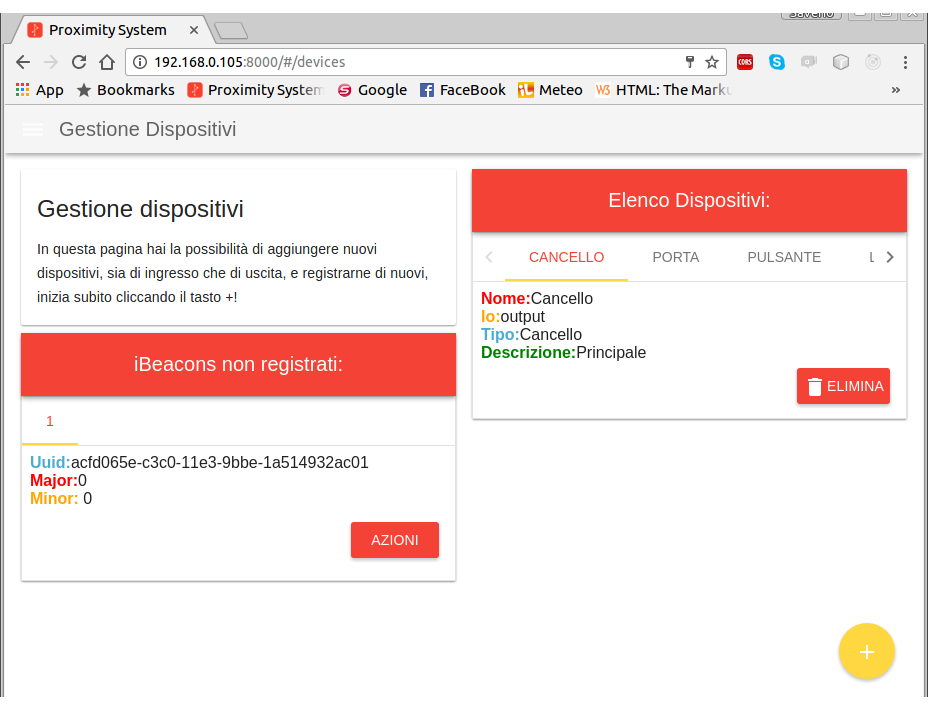
\includegraphics[width=0.8\textwidth]{dispositivi}
  \caption{Gestione dispositivi}
  \label{fig:dispositivi}
\end{figure}

\begin{figure}[htpb!]
  \centering
  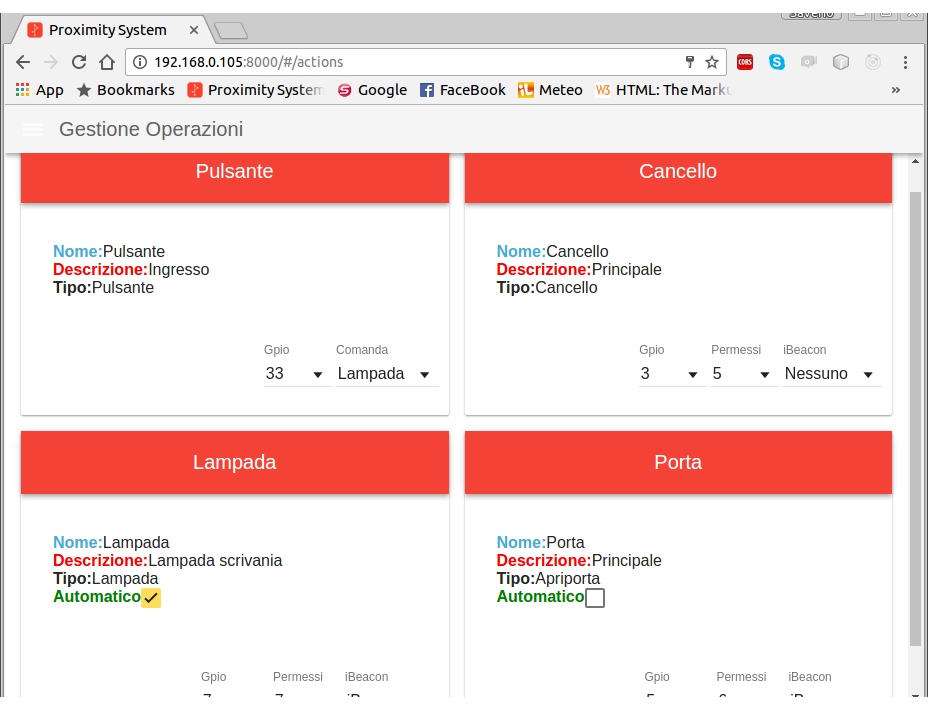
\includegraphics[width=0.8\textwidth]{operazioni}
  \caption{Gestione operazioni}
  \label{fig:operazioni}
\end{figure}
